%%%%%%%%%%%%%%%%%%%%%%%%%%%%%%%%%%%%%%%%%%%%%%%%%%%
%% LaTeX book template                           %%
%% Author:  Amber Jain (http://amberj.devio.us/) %%
%% License: ISC license                          %%
%%%%%%%%%%%%%%%%%%%%%%%%%%%%%%%%%%%%%%%%%%%%%%%%%%%
%!TEX TS-program = pdfLaTeX
%!TEX encoding = IsoLatin
%!TEX spellcheck = fr-FR

\documentclass[12pt,A4]{book}

%\documentclass[a4paper,11pt]{book}
\usepackage[T1]{fontenc}
\usepackage[utf8]{inputenc}
\usepackage[francais]{babel}

\usepackage{lmodern}
%%%%%%%%%%%%%%%%%%%%%%%%%%%%%%%%%%%%%%%%%%%%%%%%%%%%%%%%%
% Source: http://en.wikibooks.org/wiki/LaTeX/Hyperlinks %
%%%%%%%%%%%%%%%%%%%%%%%%%%%%%%%%%%%%%%%%%%%%%%%%%%%%%%%%%
\usepackage{hyperref}
\usepackage{graphicx}
\usepackage{pdfpages}
\usepackage{amsmath}
\usepackage{amssymb}
\usepackage{a4}
\usepackage{indentfirst}
\usepackage{fancyhdr}
\usepackage{varioref}
\usepackage{makeidx}

\usepackage{mslapa}

%\usepackage{apacite}
%\usepackage[longnamesfirst,nonamebreak]{natbib}

\usepackage[usenames,dvipsnames]{color}


%%%%%%%%%%%%%%%%%%%%%%%%%%%%%%%%%%%%%%%%%%%%%%%%%%%%%%%%%%%%%%%%%%%%%%%%%%%%%%
%%%%%%%%%%%%%%%%%%%%%%%%%%%%%%%%%%%%%%%%%%%%%%%%%%%%%%%%%%%%%%%%%%%%%%%%%%%%%%

\pagestyle{fancy}

\addtolength{\headwidth}{\marginparsep}
\addtolength{\headwidth}{\marginparwidth}
\renewcommand{\chaptermark}[1]{\markboth{#1}{}}
\renewcommand{\sectionmark}[1]{\markright{\thesection\ #1}}
\fancyhf{}
\fancyhead[LE,RO]{\bfseries\thepage}
\fancyhead[LO]{\bfseries\rightmark}
\fancyhead[RE]{\bfseries\leftmark}
\fancypagestyle{plain}{
\fancyhead{} % get rid of headers
\renewcommand{\headrulewidth}{0pt} % and the line
}


%% Apalike hyphenation %%%
%\let\oldbibitem=\bibitem
%\renewcommand{\bibitem}[2][]{\oldbibitem[#1]{#2}\newline}

%%% Margins %%%
\voffset -1.04cm
\textheight 23cm
\hoffset -1in
\evensidemargin 2.5cm
\oddsidemargin 2.5cm
\textwidth 16cm

%%%%%%%%%%%%%%%%%%%%%%%%%%%%%%%%%%%%%%%%%%%%%%%%%%%%%%%%%%%%%%%%%%%%%%%%%%%%%%
%%%%%%%%%%%%%%%%%%%%%%%%%%%%%%%%%%%%%%%%%%%%%%%%%%%%%%%%%%%%%%%%%%%%%%%%%%%%%%

%\textwidth16cm
%\textheight23cm
%\oddsidemargin0,5cm
%\evensidemargin0,5cm
%\topmargin-1cm
%\parskip0,5cm
%\parindent0cm



%%%%%%%%%%%%%%%%%%%%%%%%%%%%%%%%%%%%%%%%%%%%%%%%%%%%%%%%%%%%%%%%%%%%%%%%%%%%%%%%
% 'dedication' environment: To add a dedication paragraph at the start of book %
% Source: http://www.tug.org/pipermail/texhax/2010-June/015184.html            %
%%%%%%%%%%%%%%%%%%%%%%%%%%%%%%%%%%%%%%%%%%%%%%%%%%%%%%%%%%%%%%%%%%%%%%%%%%%%%%%%
\newenvironment{dedication}
{
   \cleardoublepage
   \thispagestyle{empty}
   \vspace*{\stretch{1}}
   \hfill\begin{minipage}[t]{0.66\textwidth}
   \raggedright
}
{
   \end{minipage}
   \vspace*{\stretch{3}}
   \clearpage
}

%%%%%%%%%%%%%%%%%%%%%%%%%%%%%%%%%%%%%%%%%%%%%%%%
% Chapter quote at the start of chapter        %
% Source: http://tex.stackexchange.com/a/53380 %
%%%%%%%%%%%%%%%%%%%%%%%%%%%%%%%%%%%%%%%%%%%%%%%%
\makeatletter
\renewcommand{\@chapapp}{}% Not necessary...
\newenvironment{chapquote}[2][2em]
  {\setlength{\@tempdima}{#1}%
   \def\chapquote@author{#2}%
   \parshape 1 \@tempdima \dimexpr\textwidth-2\@tempdima\relax%
   \itshape}
  {\par\normalfont\hfill--\ \chapquote@author\hspace*{\@tempdima}\par\bigskip}
\makeatother


% Babel ``Sommaire'' à la place de ``table des matières''
\renewcommand{\contentsname}{Sommaire}


%%%%%%%%%%%%%%%%%%%%%%%%%%%%%%%%%%%%%%%%%%%%%%%%%%%
% First page of book which contains 'stuff' like: %
%  - Book title, subtitle                         %
%  - Book author name                             %
%%%%%%%%%%%%%%%%%%%%%%%%%%%%%%%%%%%%%%%%%%%%%%%%%%%

% Book's title and subtitle
\title{\Huge \textbf{Apprentissage dans les architectures cognitives}  \\ \vspace{1cm} \huge Contributions pour l'informatique et les neurosciences \\ \vspace{1cm} \Large \emph{Documents annexes}}
% Author
\author{\textsc{Emmanuel Daucé}}%\thanks{\url{www.example.com}}}


\begin{document}

\frontmatter
\maketitle

%%%%%%%%%%%%%%%%%%%%%%%%%%%%%%%%%%%%%%%%%%%%%%%%%%%%%%%%%%%%%%%
% Add a dedication paragraph to dedicate your book to someone %
%%%%%%%%%%%%%%%%%%%%%%%%%%%%%%%%%%%%%%%%%%%%%%%%%%%%%%%%%%%%%%%
%\begin{dedication}
%Dedicated to Calvin and Hobbes.
%\end{dedication}

%%%%%%%%%%%%%%%%%%%%%%%%%%%%%%%%%%%%%%%%%%%%%%%%%%%%%%%%%%%%%%%%%%%%%%%%
% Auto-generated table of contents, list of figures and list of tables %
%%%%%%%%%%%%%%%%%%%%%%%%%%%%%%%%%%%%%%%%%%%%%%%%%%%%%%%%%%%%%%%%%%%%%%%%
\tableofcontents
%\listoffigures
%\listoftables

\mainmatter

%\section*{Remerciements}
%\begin{itemize}
%\item A special word of thanks goes to Professor Don Knuth\footnote{\url{http://www-cs-faculty.stanford.edu/~uno/}} (for \TeX{}) and Leslie Lamport\footnote{\url{http://www.lamport.org/}} (for \LaTeX{}).
%\item I'll also like to thank Gummi\footnote{\url{http://gummi.midnightcoding.org/}} developers and LaTeXila\footnote{\url{http://projects.gnome.org/latexila/}} development team for their awesome \LaTeX{} editors.
%\item I'm deeply indebted my parents, colleagues and friends for their support and encouragement.
%\end{itemize}
%\mbox{}\\
%\mbox{}\\
%\noindent Amber Jain \\
%\noindent \url{http://amberj.devio.us/}

%%%%%%%%%%%%%%%%
% NEW CHAPTER! %
%%%%%%%%%%%%%%%%


%%%%%%%%%%%%%%%%%%%%%%%%%%%%%%%%%%%%%%%%%%%%%%%%%%%%%%%%%%%%%%%%%%%%%%%%%%%%%%%%%%%%%%%%%%%%%%%%%%%%%%%%%%%%%%%%%%%
%%%%%%%%%%%%%%%%%%%%%%%%%%%%%%%%%%%%%%%%%%%%%%%%%%%%%%%%%%%%%%%%%%%%%%%%%%%%%%%%%%%%%%%%%%%%%%%%%%%%%%%%%%%%%%%%%%%
%%%%%%%%%%%%%%%%%%%%%%%%%%%%%%%%%%%%%%%%%%%%%%%%%%%%%%%%%%%%%%%%%%%%%%%%%%%%%%%%%%%%%%%%%%%%%%%%%%%%%%%%%%%%%%%%%%%
%%%%%%%%%%%%%%%%%%%%%%%%%%%%%%%%%%%%%%%%%%%%%%%%%%%%%%%%%%%%%%%%%%%%%%%%%%%%%%%%%%%%%%%%%%%%%%%%%%%%%%%%%%%%%%%%%%%
%%%%%%%%%%%%%%%%%%%%%%%%%%%%%%%%%%%%%%%%%%%%%%%%%%%%%%%%%%%%%%%%%%%%%%%%%%%%%%%%%%%%%%%%%%%%%%%%%%%%%%%%%%%%%%%%%%%
%%%%%%%%%%%%%%%%%%%%%%%%%%%%%%%%%%%%%%%%%%%%%%%%%%%%%%%%%%%%%%%%%%%%%%%%%%%%%%%%%%%%%%%%%%%%%%%%%%%%%%%%%%%%%%%%%%%


\chapter{Neurocomputing (2007)}

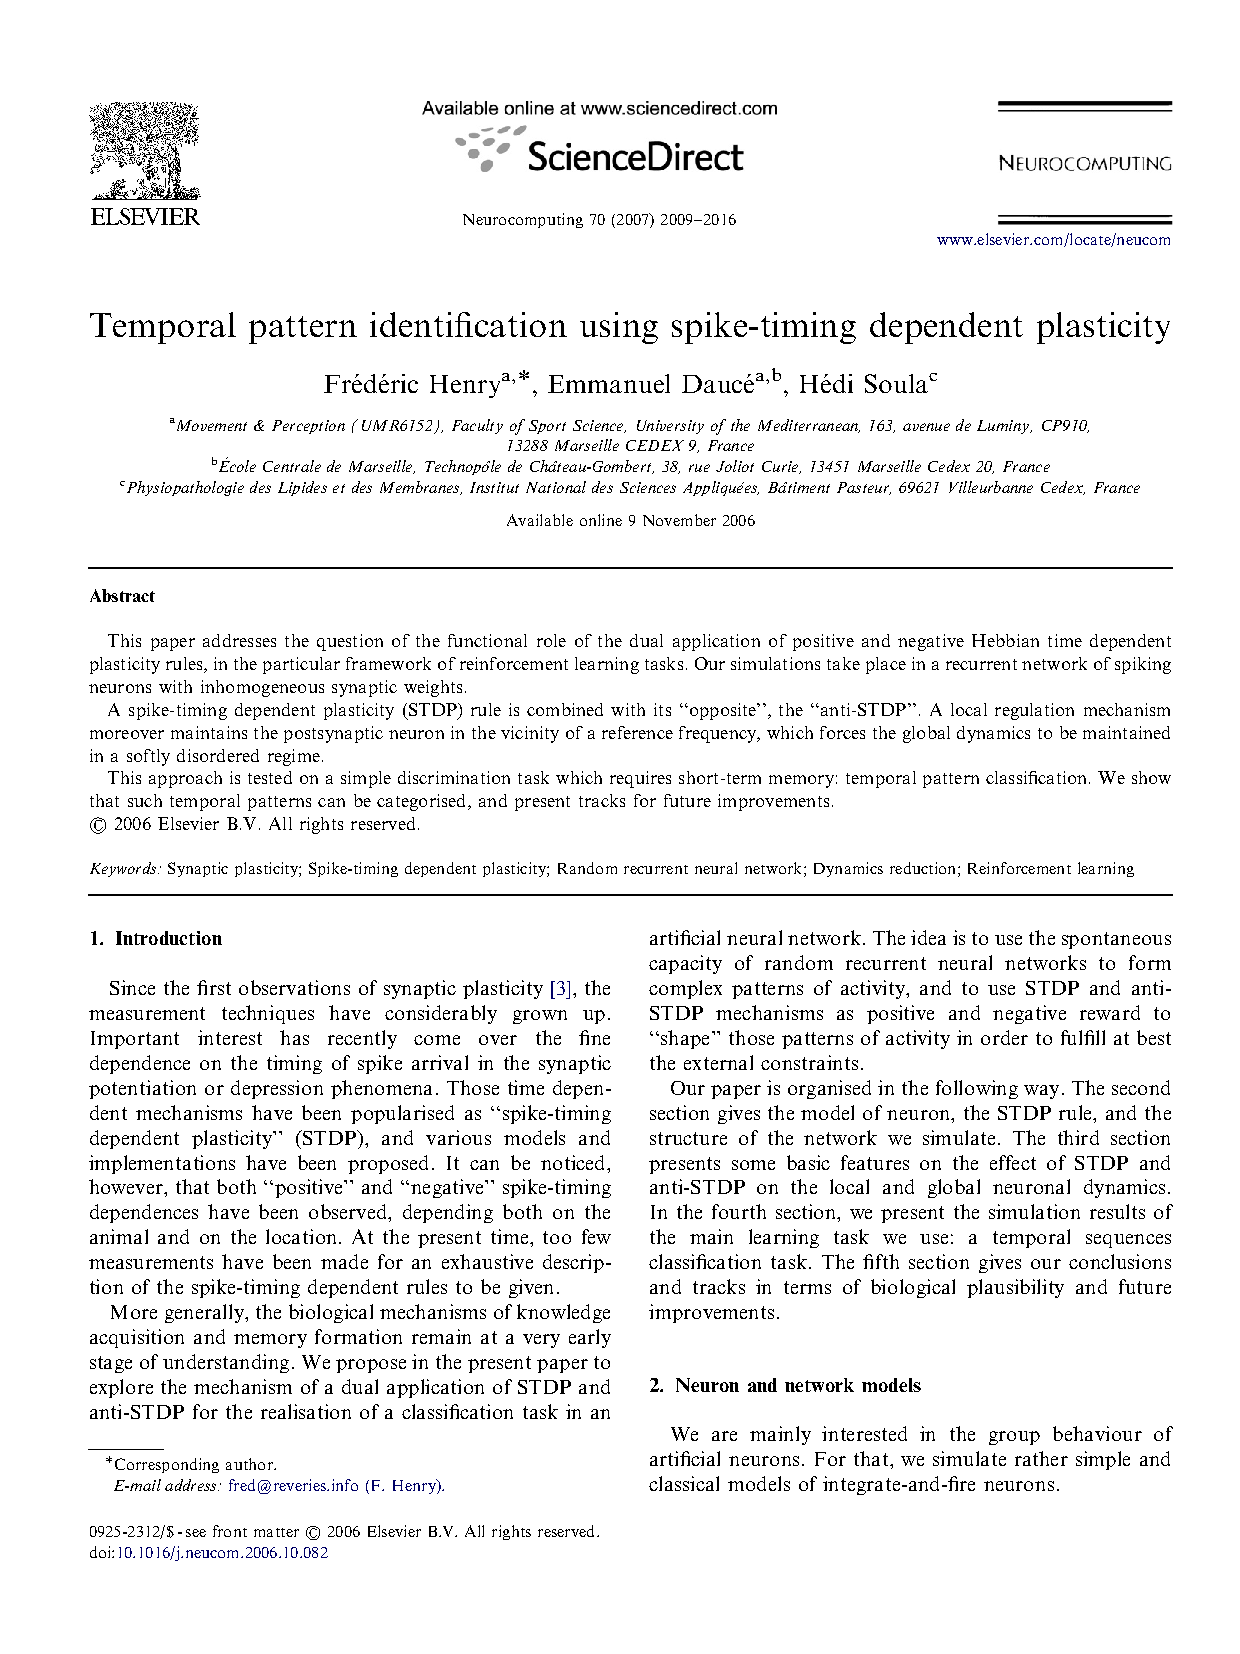
\includepdf[pages=1-8,scale=1]{pdf/neurocomputing-2007.pdf}

\chapter{European Physical Journal - Special Topics (2007)}
% \bibitem[\protect\citeauthoryear{Dauc\'e}{Dauc\'e}{2007}{}]{Dau07}
% Dauc\'e, E. (2007).
% \newblock Learning an control with large dynamic neural networks.
% \newblock {\em European Physical Journal - Special Topics}, {\em 142(1)},
%   123--161.
  
%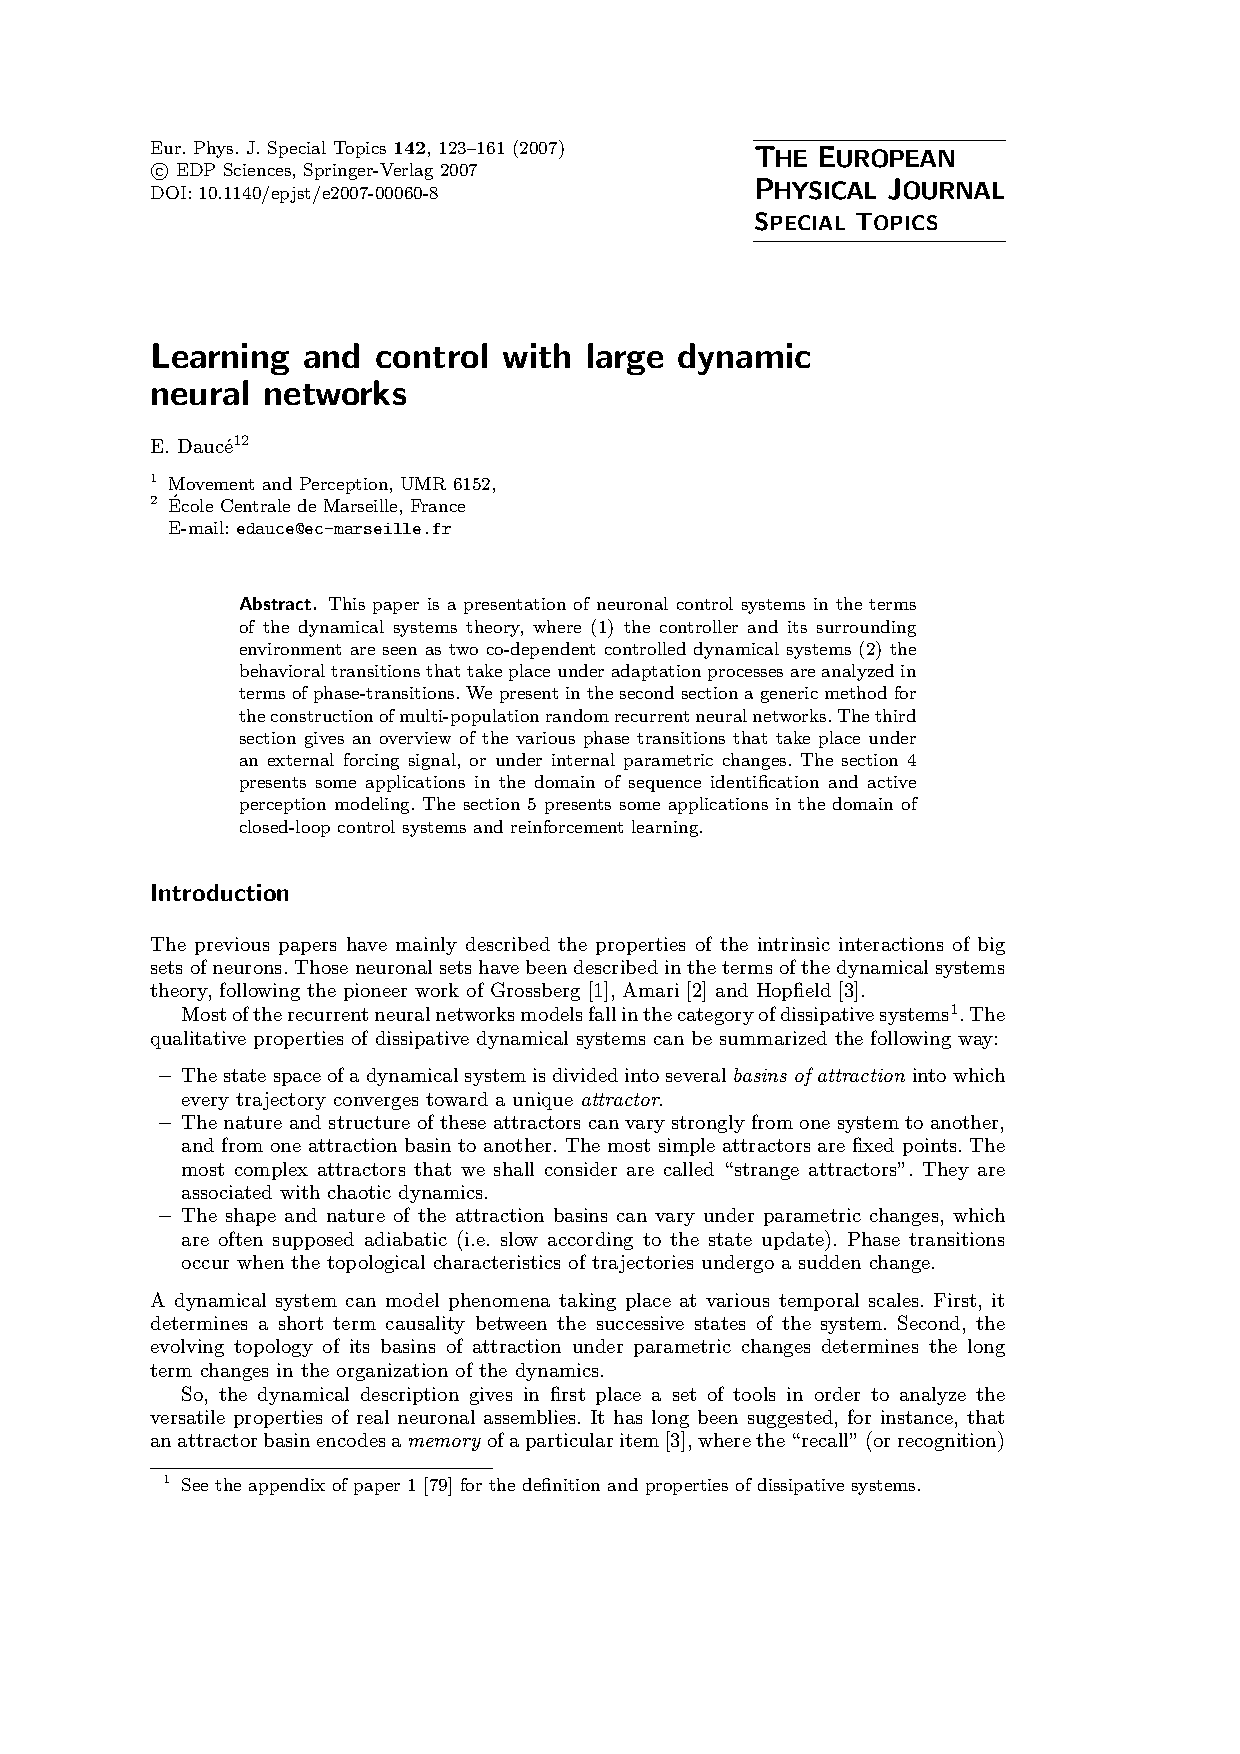
\includepdf[pages=1-10]{pdf/epj-st-2007.pdf}
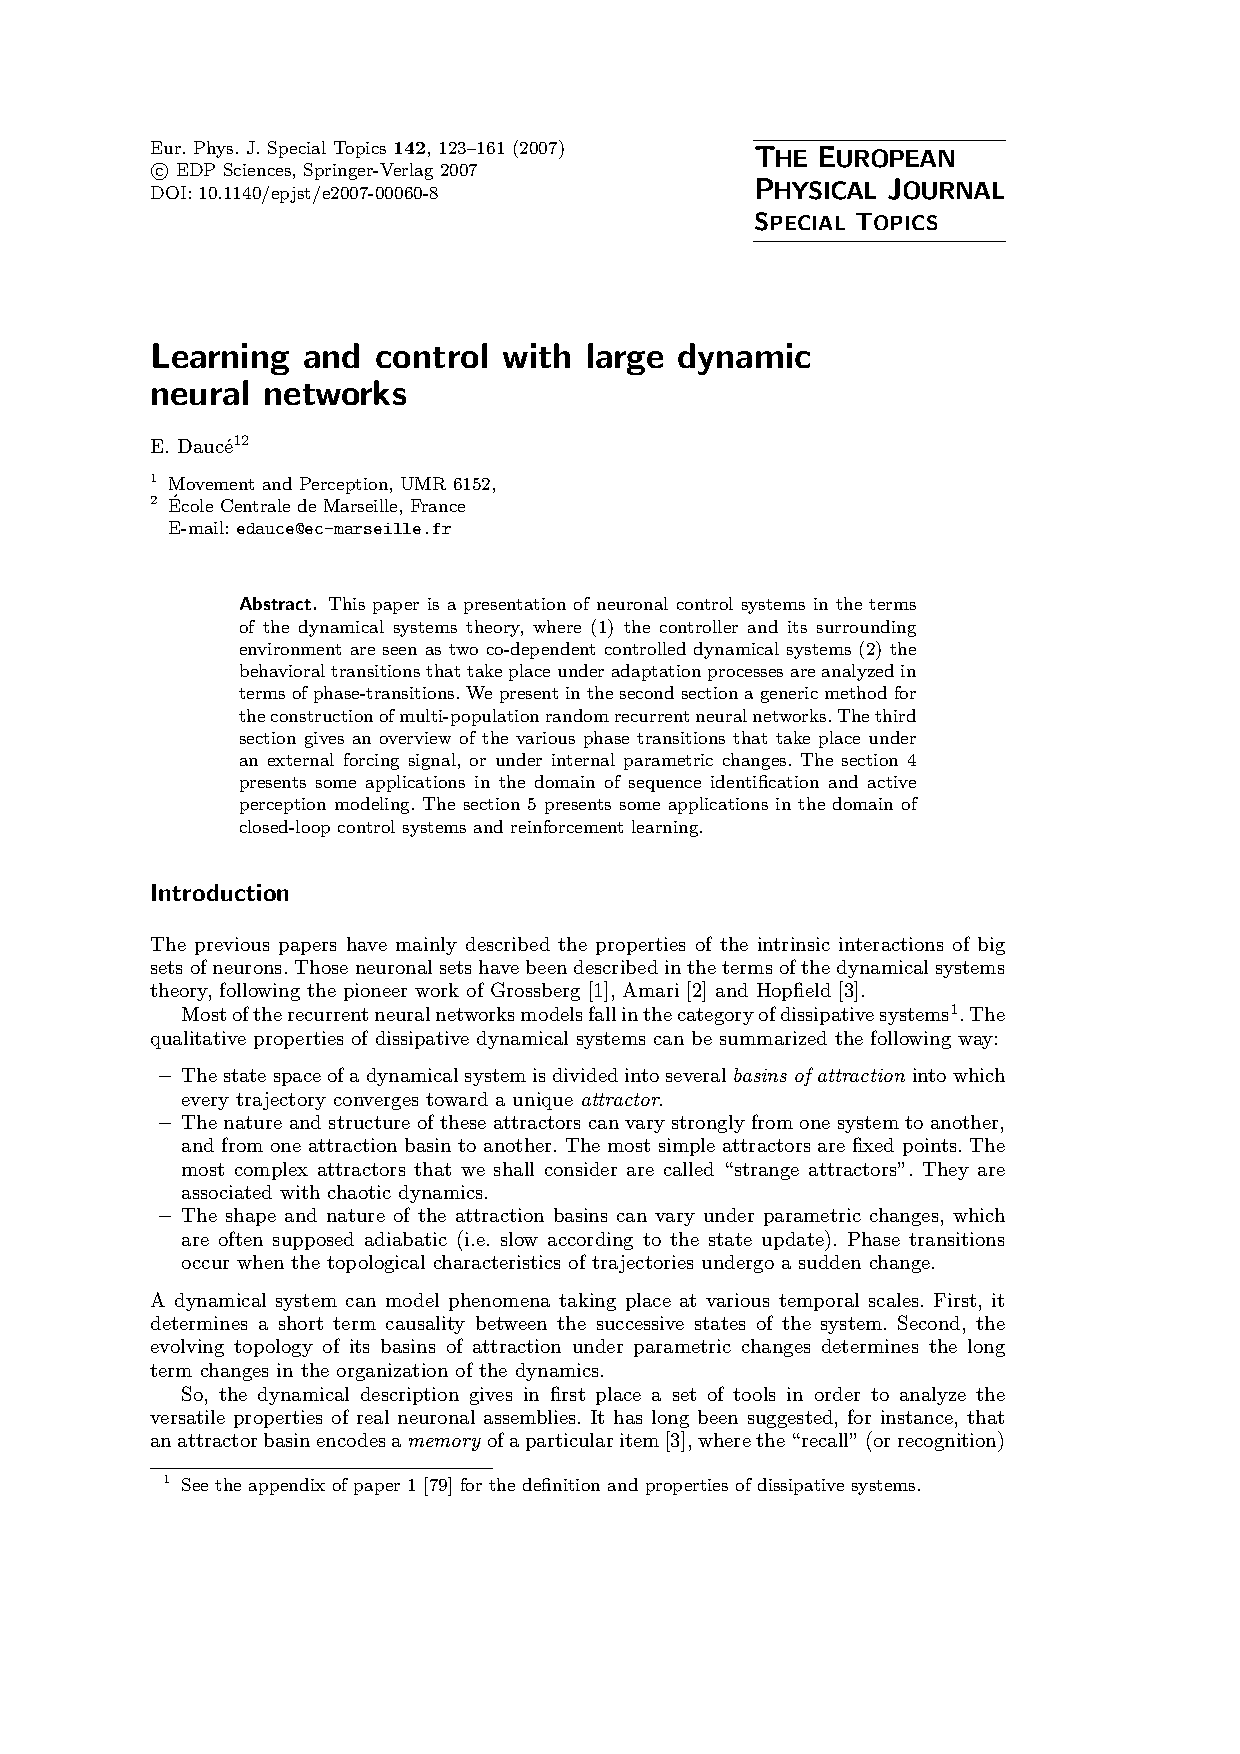
\includepdf[pages=1-40]{pdf/epj-st-2007.pdf}

\chapter{Natural Computing (2004)}
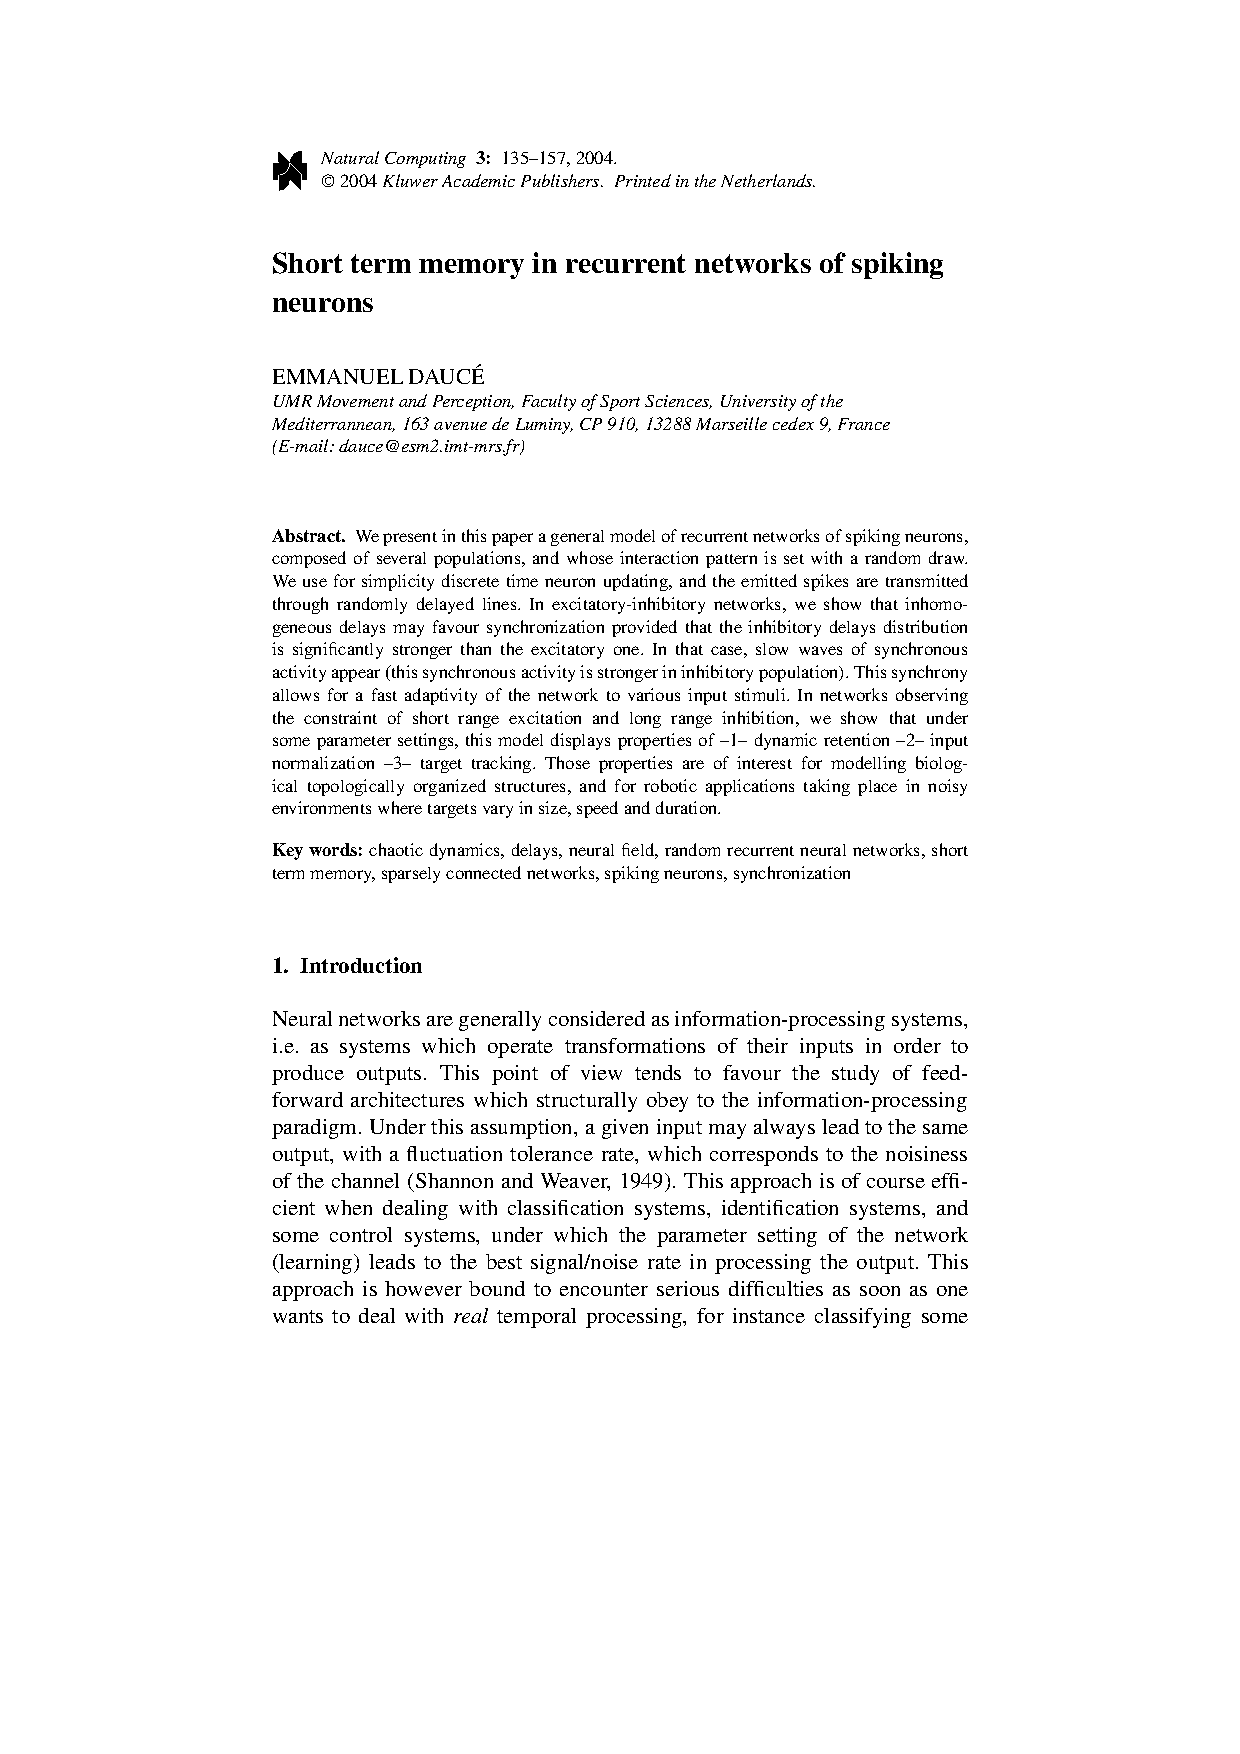
\includepdf[pages=1-24,scale=1]{pdf/natural-computing-2004.pdf}
% 
\chapter{Biological Cybernetics (2002)}
%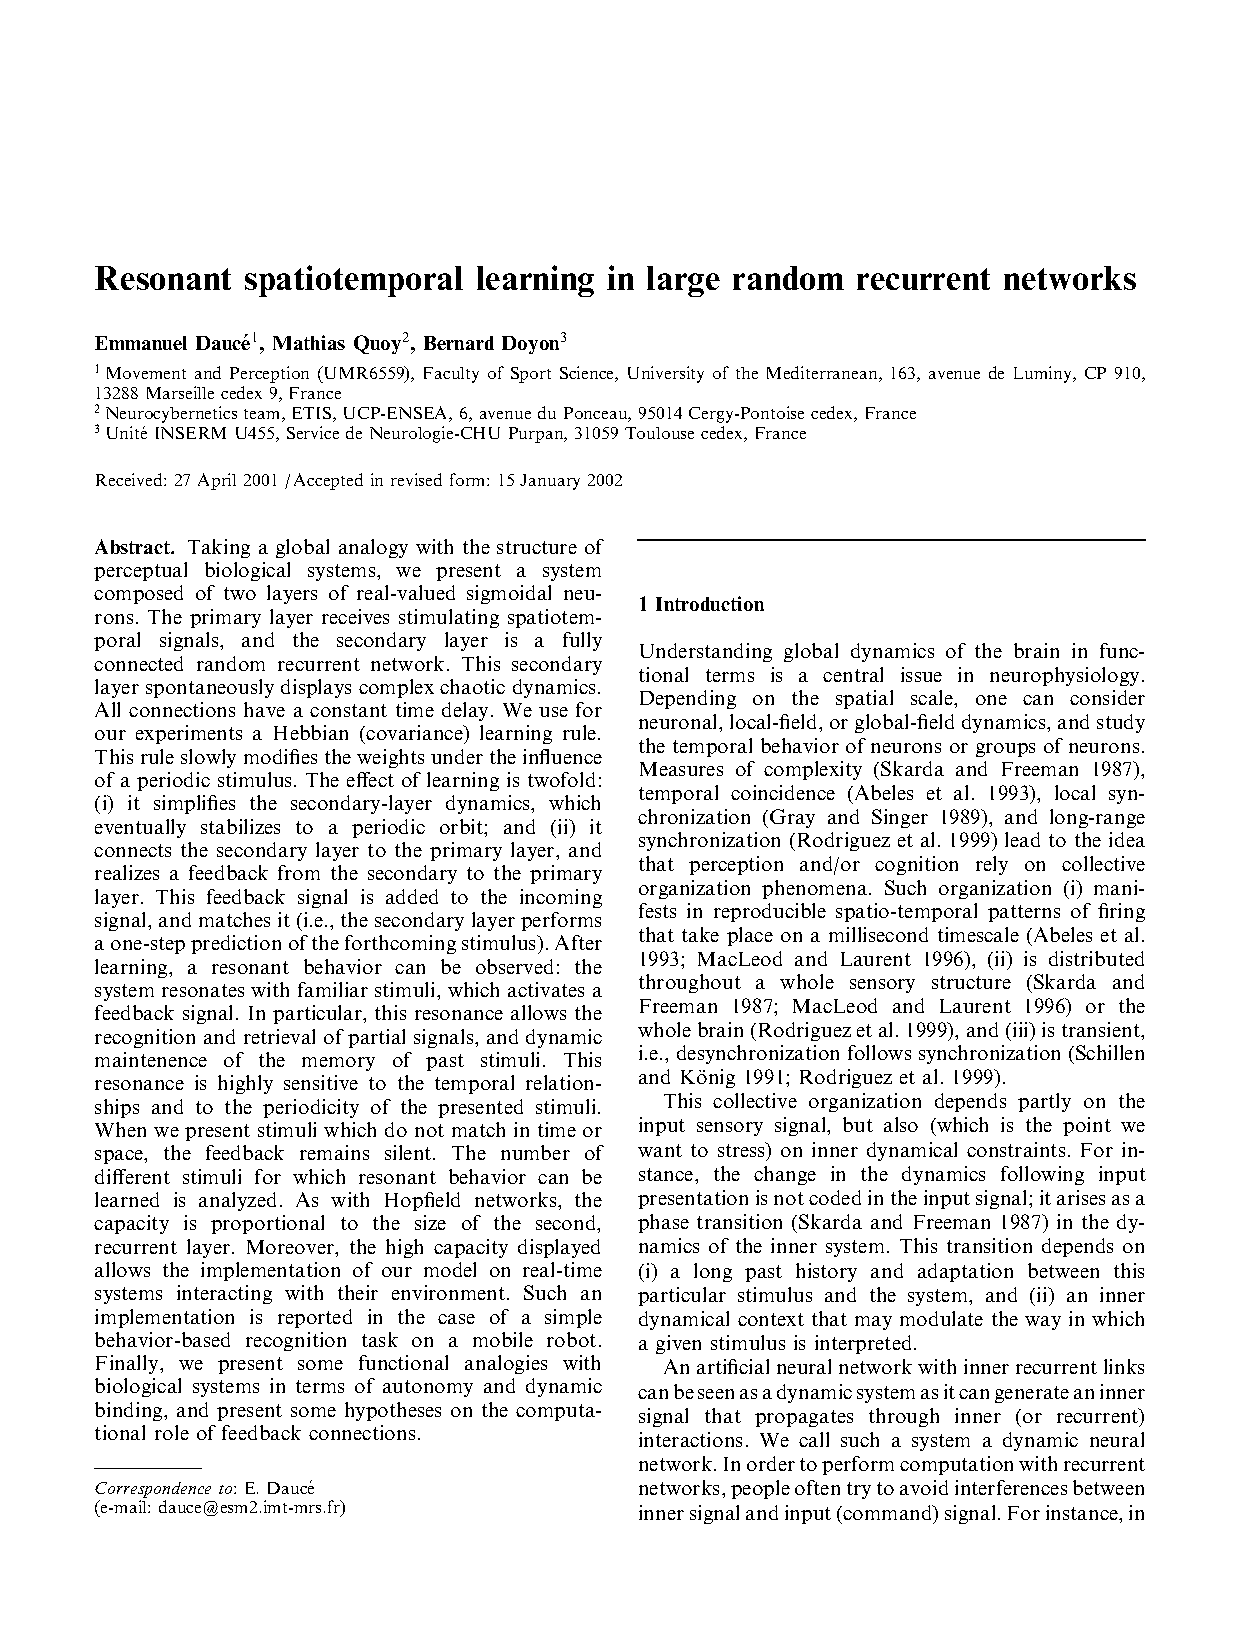
\includepdf[pages=-,templatesize={170mm}{250mm}, frame=true, openright=true, noautoscale=true]{pdf/biological-cyb-2002.pdf}
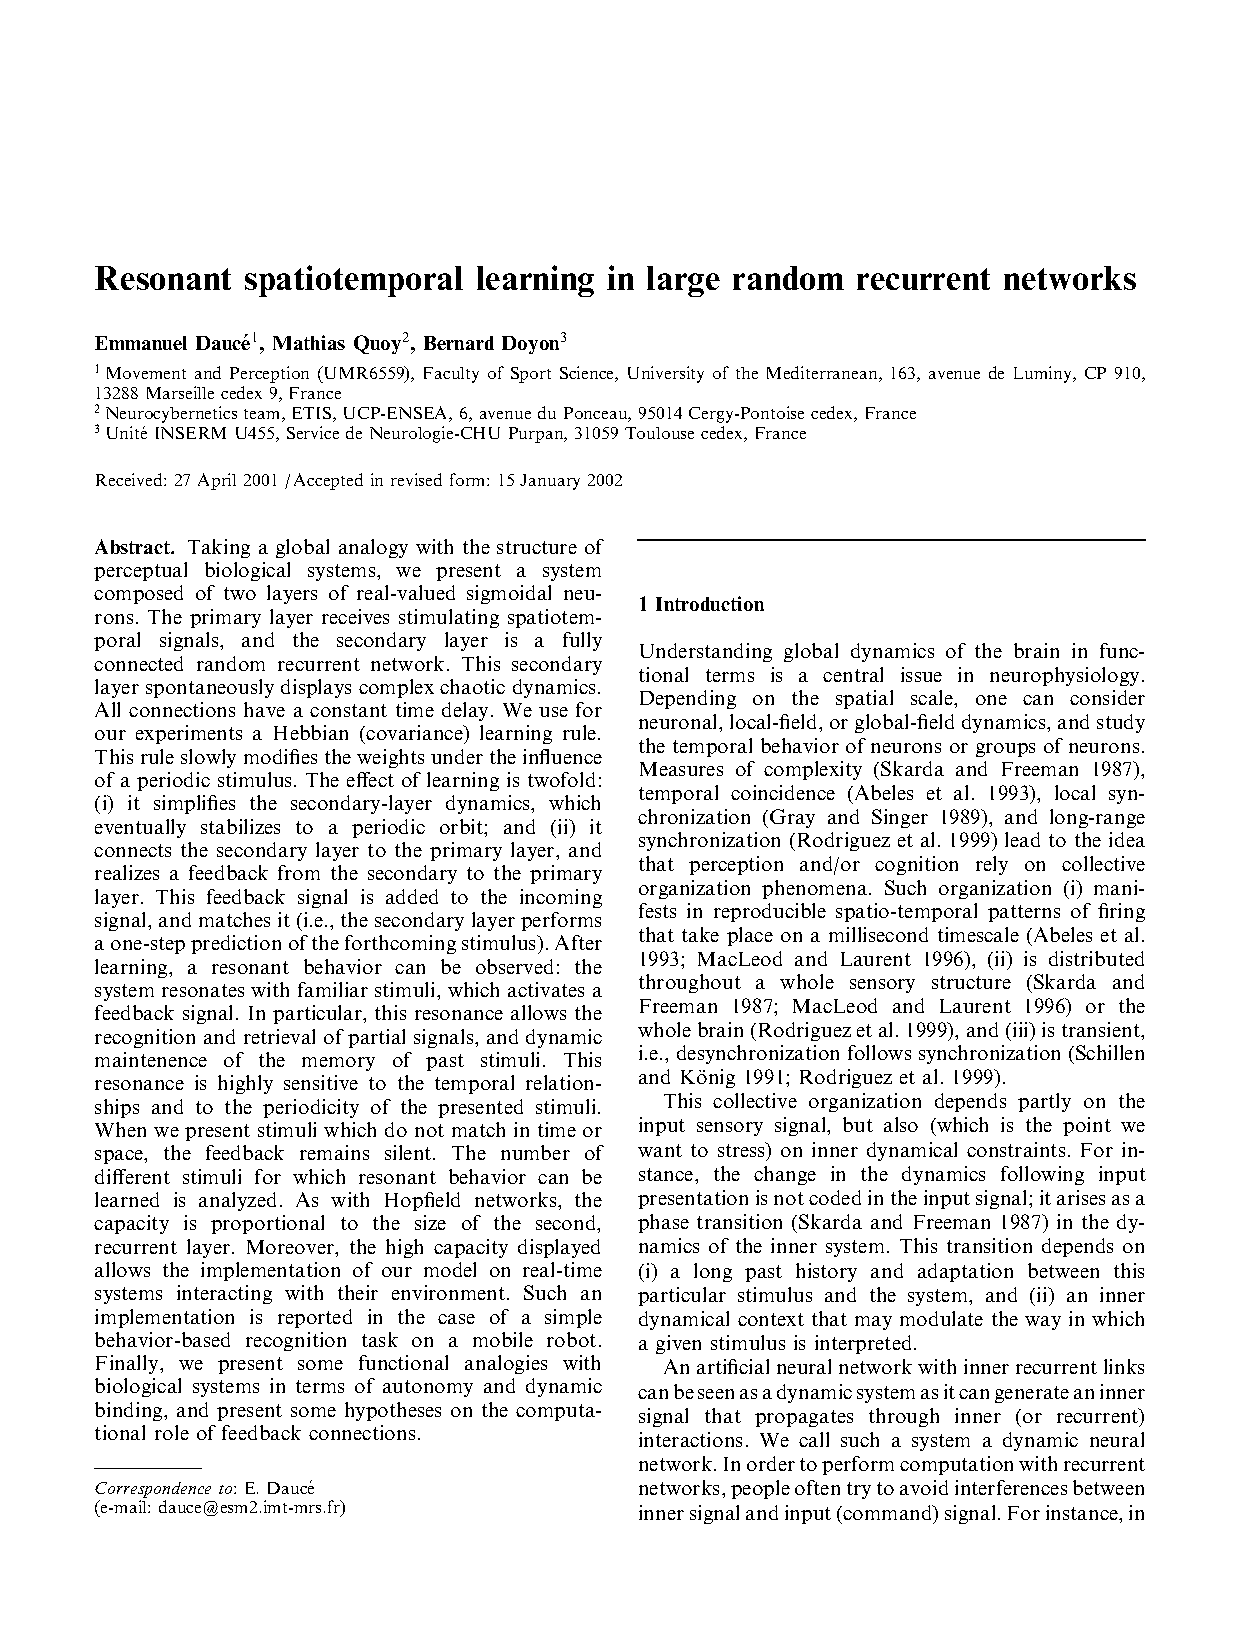
\includepdf[pages=-, scale=.8, frame=true, openright=true, noautoscale=true, offset=40 0]{pdf/biological-cyb-2002.pdf}
%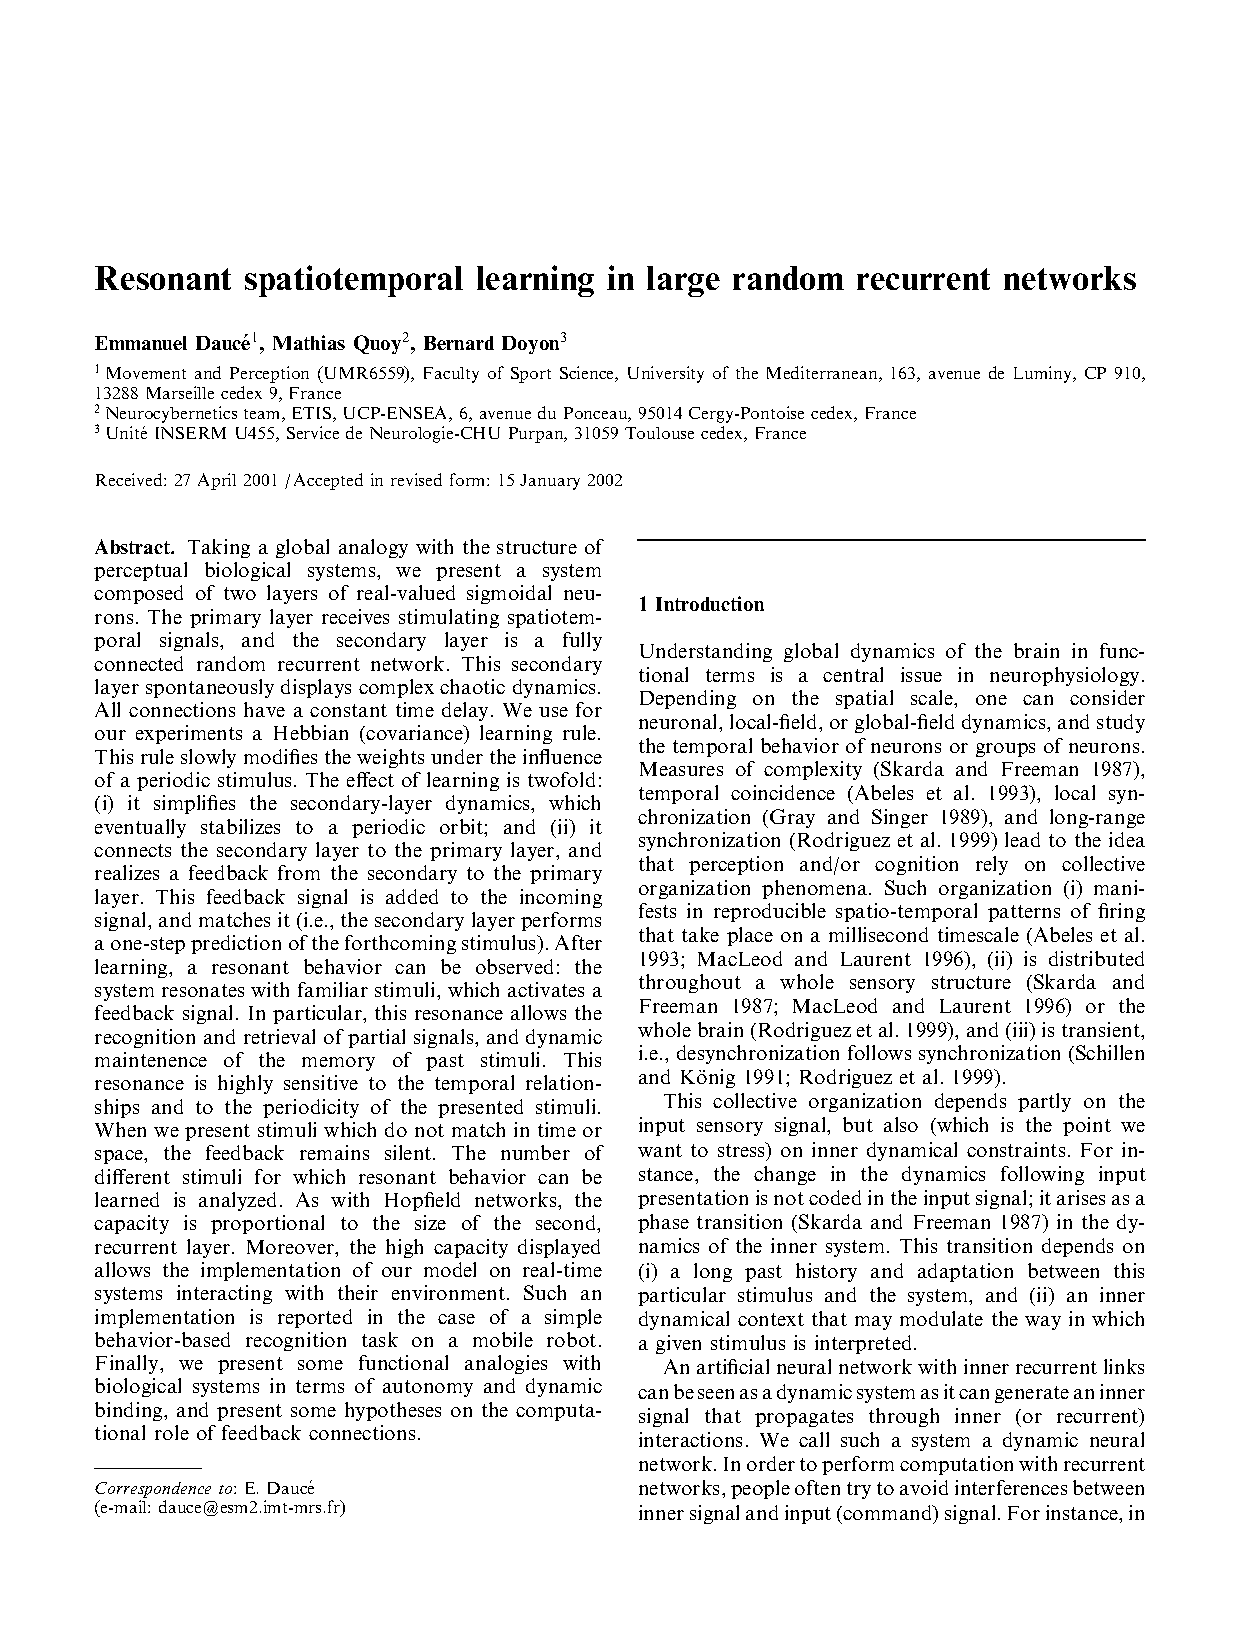
\includepdf[pages=-,,,frame=true]{pdf/biological-cyb-2002.pdf}

\chapter{Neural Processing Letters (2001)}
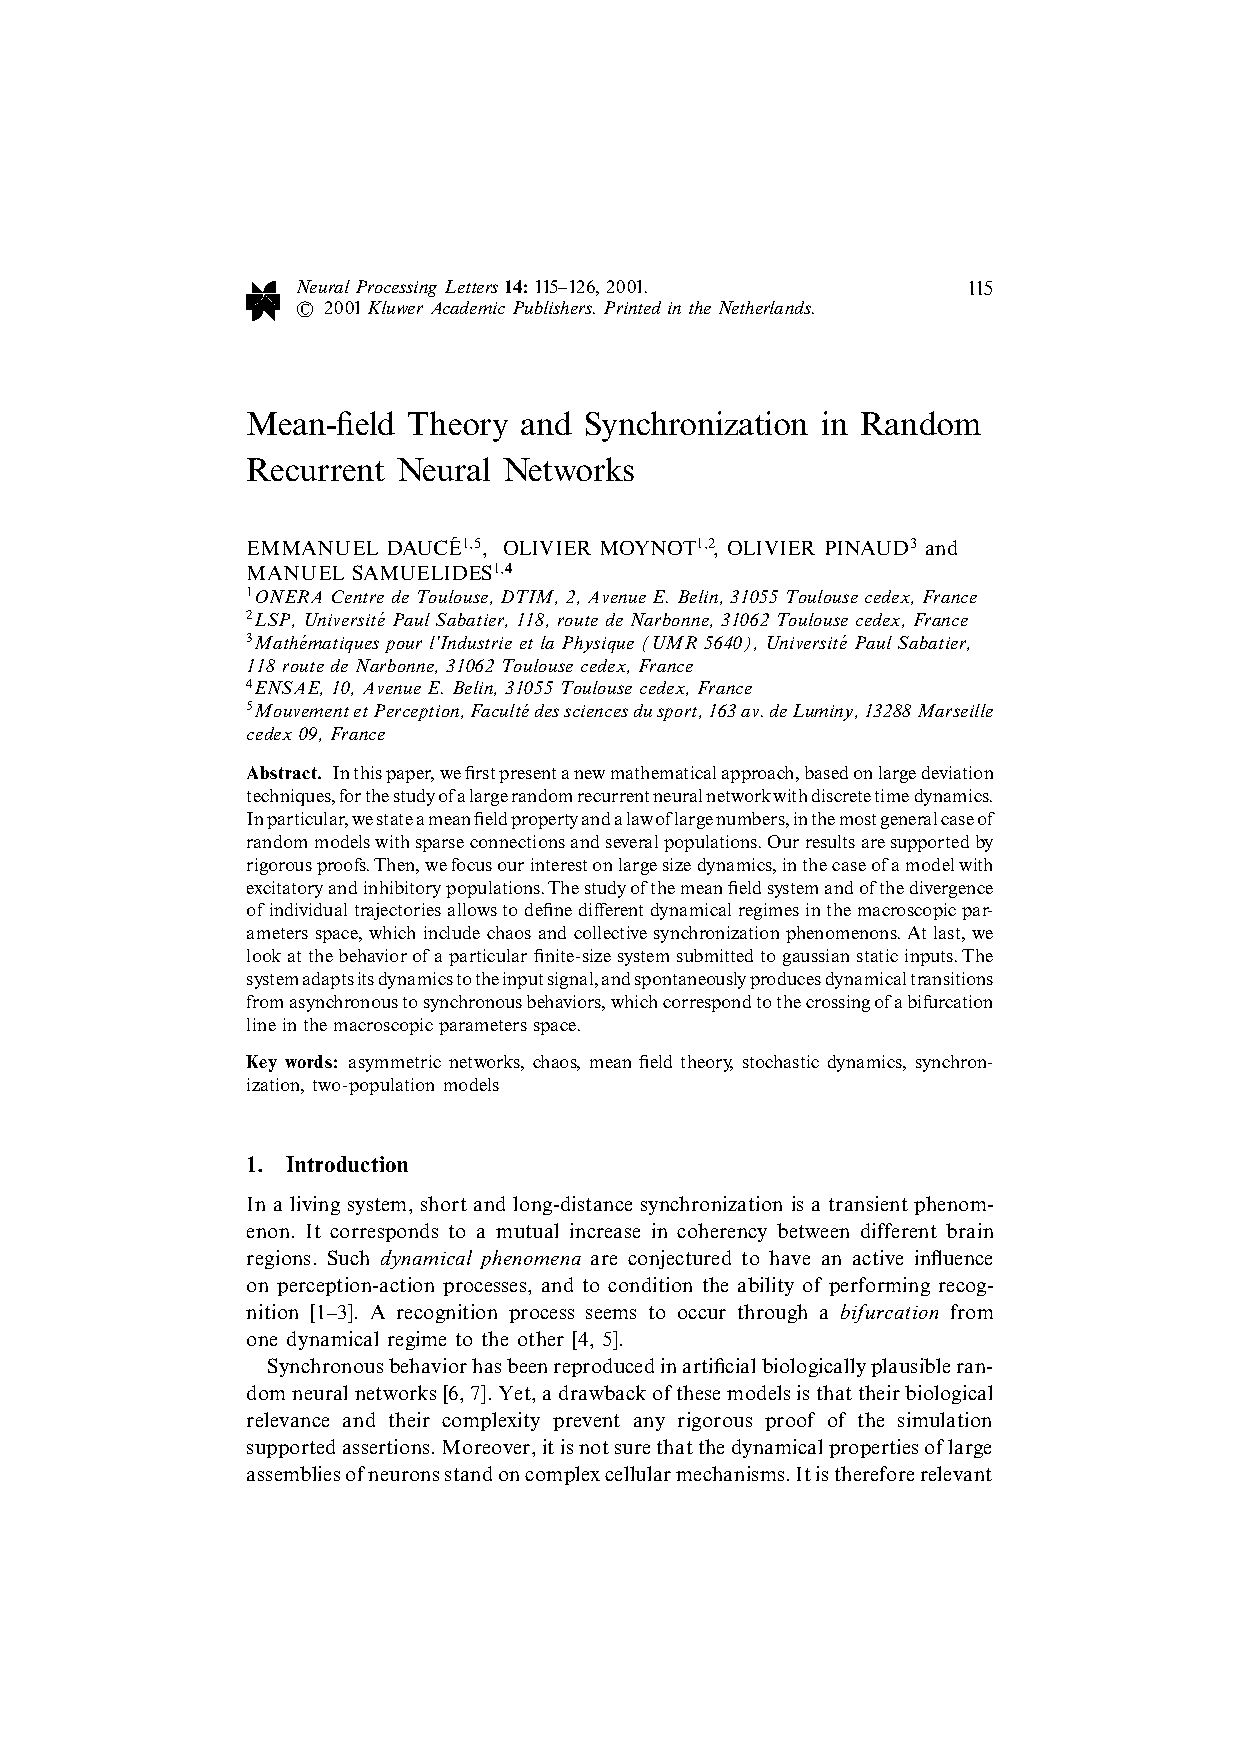
\includepdf[pages=1-12,scale=1]{pdf/neural-proc-letters-2001.pdf}

\chapter{Neural Networks (1998)}
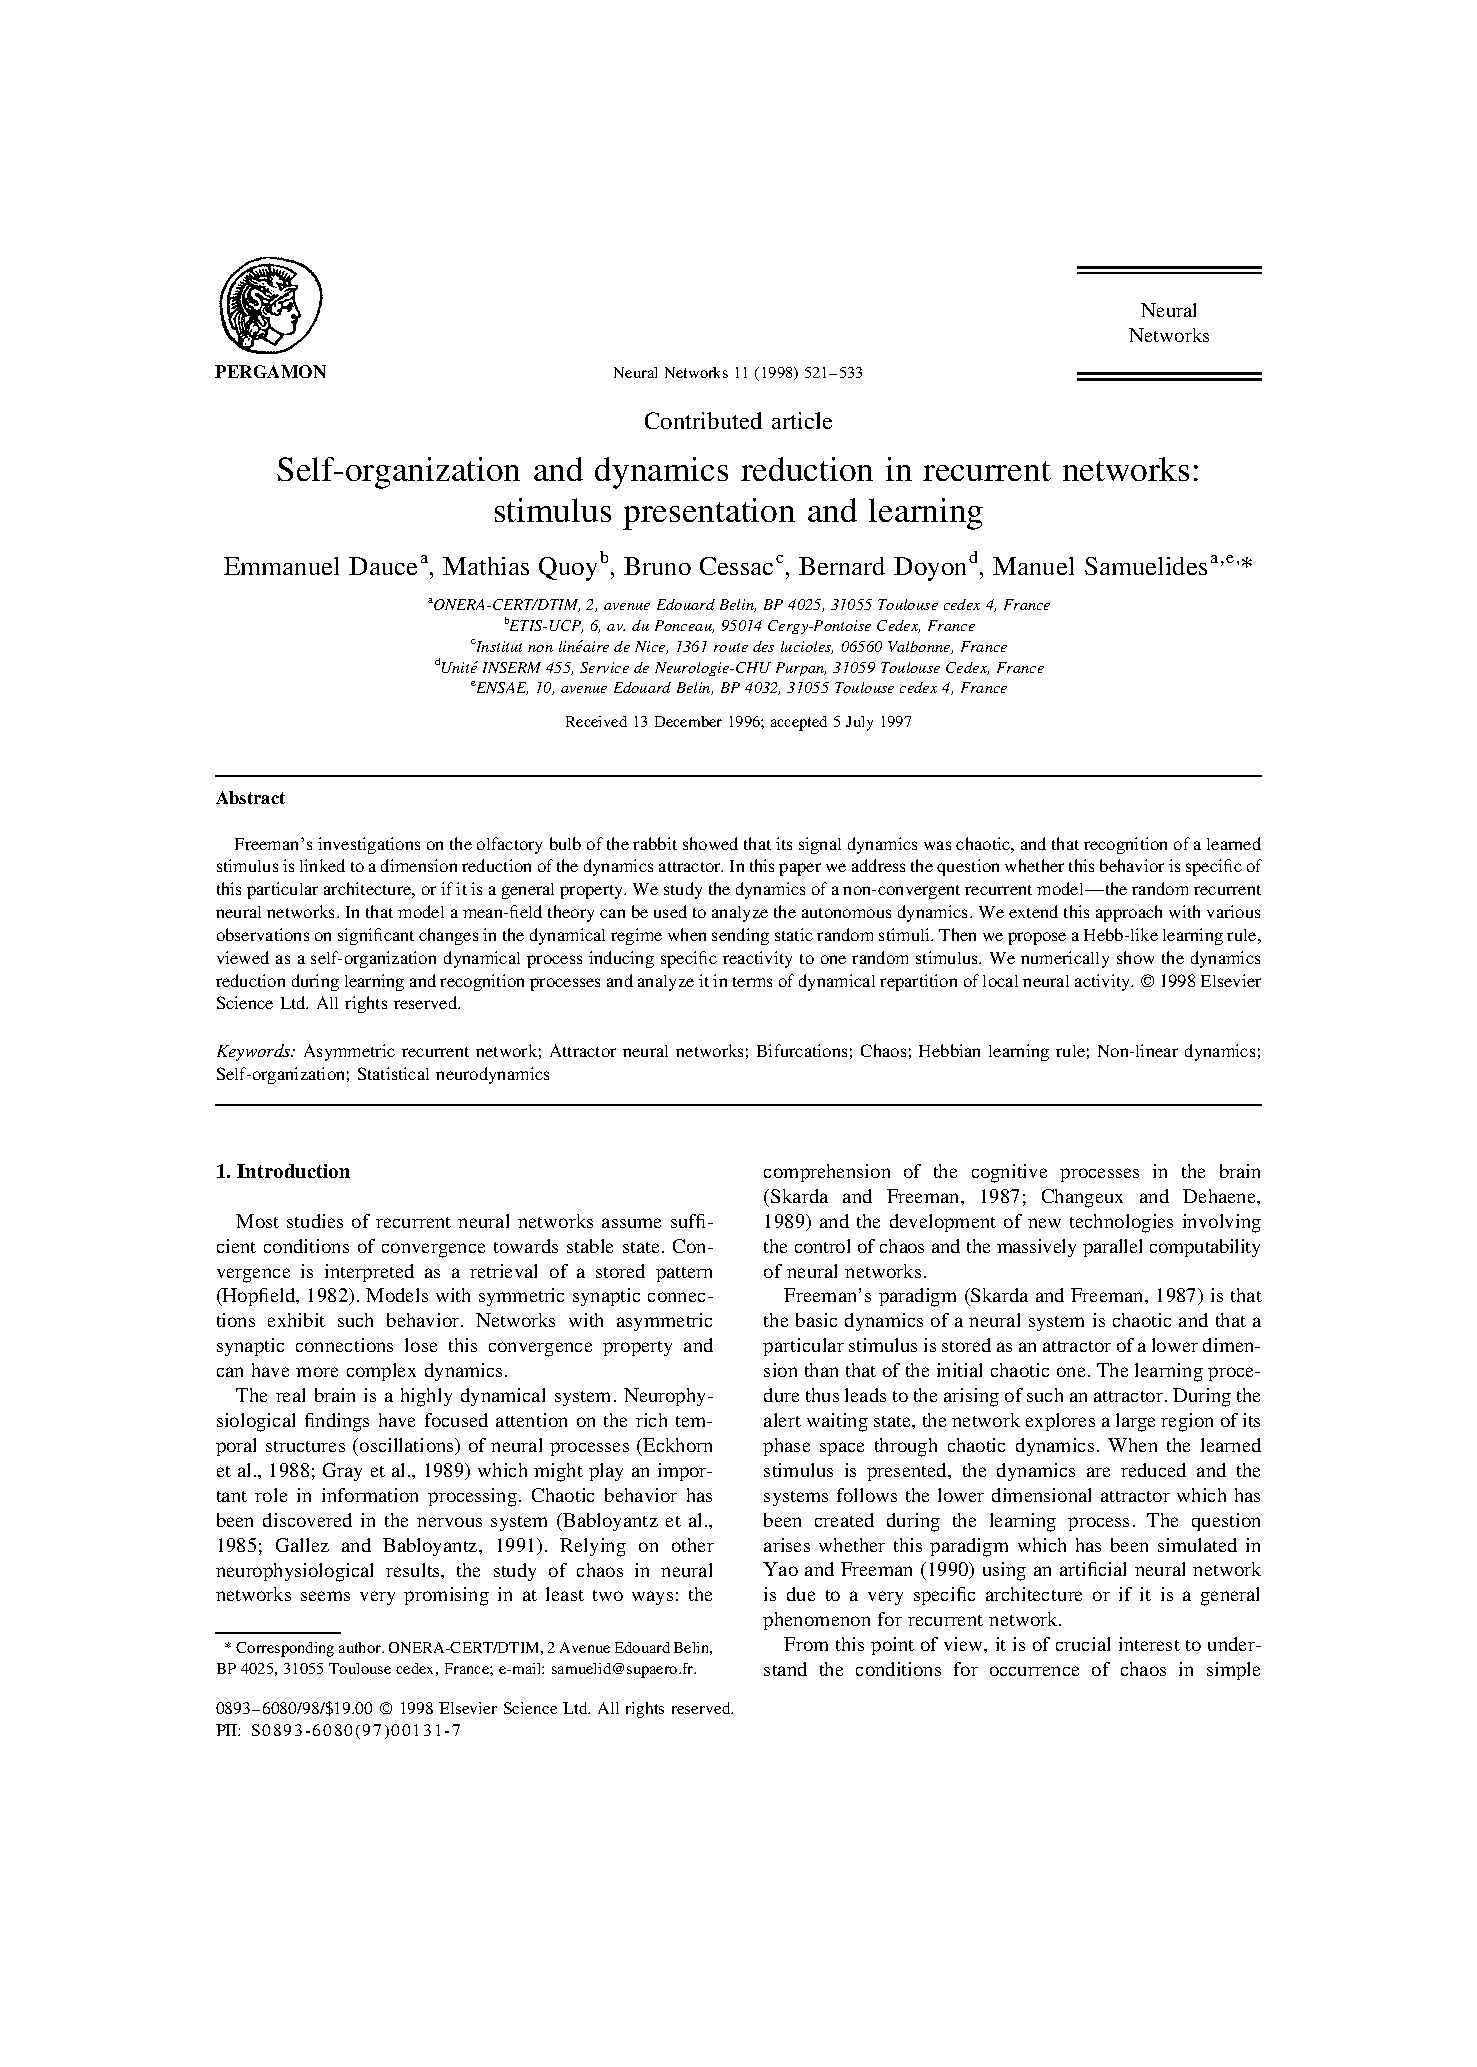
\includepdf[pages=1-13,scale=1]{pdf/neural-networks-1998.pdf}

\bibliographystyle{mslapa}%{apalike}%{apacite}
\bibliography{biblio}


\end{document}
